\documentclass[8pt, landscape]{extarticle}
\usepackage[scaled=0.92]{helvet}
\usepackage{calc}
\usepackage{multicol}
\usepackage[a4paper,margin=3mm,landscape]{geometry}
\usepackage{amsmath,amsthm,amsfonts,amssymb}
\usepackage{color,graphicx,overpic}
\usepackage{hyperref}
\usepackage{newtxtext} 
\usepackage{enumitem}
\usepackage[table]{xcolor}
\usepackage{mathtools}
\usepackage{caption}
\usepackage{subfig}

\setlist{nosep}
% for including images
\graphicspath{ {./images/} }

\pdfinfo{
  /Title (CS3223.pdf)
  /Creator (TeX)
  /Producer (pdfTeX 1.40.0)
  /Author (Jovyn Tan, Jotham Wong)
  /Subject (CS3223)
/Keywords (CS3223, nus,cheatsheet,pdf)}

% Turn off header and footer
\pagestyle{empty}

% redefine section commands to use less space
\makeatletter
\renewcommand{\section}{\@startsection{section}{1}{0mm}%
  {-1ex plus -.5ex minus -.2ex}%
  {0.5ex plus .2ex}%x
{\normalfont\large\bfseries}}
\renewcommand{\subsection}{\@startsection{subsection}{2}{0mm}%
  {-1explus -.5ex minus -.2ex}%
  {0.5ex plus .2ex}%
{\normalfont\normalsize\bfseries}}
\renewcommand{\subsubsection}{\@startsection{subsubsection}{3}{0mm}%
  {-1ex plus -.5ex minus -.2ex}%
  {1ex plus .2ex}%
{\normalfont\small\bfseries}}%
\makeatother

\renewcommand{\familydefault}{\sfdefault}
\renewcommand\rmdefault{\sfdefault}
%  makes nested numbering (e.g. 1.1.1, 1.1.2, etc)
\renewcommand{\labelenumii}{\theenumii}
\renewcommand{\theenumii}{\theenumi.\arabic{enumii}.}
\renewcommand\labelitemii{•}
\renewcommand\labelitemiii{•}

\definecolor{mathblue}{cmyk}{1,.72,0,.38}
\everymath\expandafter{\the\everymath \color{mathblue}}

% Don't print section numbers
\setcounter{secnumdepth}{0}

\setlength{\parindent}{0pt}
\setlength{\parskip}{0pt plus 0.5ex}
%% adjust spacing for all itemize/enumerate
\setlength{\leftmargini}{0.5cm}
\setlength{\leftmarginii}{0.5cm}
\setlist[itemize,1]{leftmargin=2mm,labelindent=1mm,labelsep=1mm}
\setlist[itemize,2]{leftmargin=4mm,labelindent=1mm,labelsep=1mm}
\setlist[itemize,3]{leftmargin=4mm,labelindent=1mm,labelsep=1mm}

\captionsetup{belowskip=0pt}
% adding my commands
% tightcenter
\newenvironment{tightcenter}{%
  \setlength\topsep{0pt}
  \setlength\parskip{0pt}
  \begin{center}
    }{%
  \end{center}
}

% boxed
\newenvironment{tightbox}{%
  \setlength\topsep{0pt}
  \setlength\parskip{0pt}
  \begin{center}
    \begin{tabular}{|@{\hspace{\dimexpr\fboxsep+0.5\arrayrulewidth}}c@{\hspace{\dimexpr\fboxsep+0.5\arrayrulewidth}}|}
      \hline
    }
    {%
    \\ \hline
    \end{tabular}
  \end{center}
}

% fixed width box
\newenvironment{fixedbox}[1][0.7]{
  \setlength\topsep{0pt}
  \setlength\parskip{0pt}
  \begin{center}
    \begin{tabular}{|>{\centering\arraybackslash}m{#1\linewidth}|}
    \hline
  }{
  \\ \hline
  \end{tabular}
  \end{center}
}

% definition of a new term
\usepackage{soul}
\definecolor{paleyellow}{RGB}{251,243,218}
\newcommand{\definition}[2][]{\sethlcolor{paleyellow}\hl{\textbf{#2}} #1  $\rightarrow$}
% inline definition
\newcommand{\ildefinition}[1]{\sethlcolor{paleyellow}\hl{\textbf{#1}}}

% important note (attention)
\newcommand{\attention}{{\color{red}\textbf{! }}}

% nice proof
\newenvironment{niceproof}[1][Proof]
{%
  \sbox0{\textit{#1}. }%
  \list{}{\labelwidth\wd0 \leftmargin\wd0 \labelsep 0pt }
\item[\usebox0]}
  {\endlist}



% -----------------------------------------------------------------------

\begin{document}
\raggedright
\footnotesize
\begin{multicols*}{4}
  % multicol parameters
  \setlength{\columnseprule}{0.25pt}

  \begin{center}
    \fbox{%
      \parbox{0.8\linewidth}{\centering \textcolor{black}{
          {\Large\textbf{COS375}}
        \\ \normalsize{Fall 2023}}
        \\ {\footnotesize \textcolor{gray}{github/jovyntls github/JothamWong}}
      }%
    }
  \end{center}

  \section{Instruction Set Architecture}
  \begin{itemize}
    \item Architecture: Abstraction layer provided to SW to interface with HW.
      \begin{itemize}
        \item Examples: ARM, x86, MIPS
        \item Designed for stability and to hide implementation details.
        \item Includes programmer visible state/operations/instructions/data types/sizes/execution semantics.
      \end{itemize}
      \item Microarchitecture: Physical instance of contract. Implementation details.
      \begin{itemize}
        \item Includes additional state not visible to programmer such as cache size.
      \end{itemize}
      \item Design goals
      \begin{enumerate}
        \item Portability
        \item Programmability
        \item Efficiency (power/energy/speed/code size/cost)
      \end{enumerate}
    \end{itemize}
    
    \subsection{MIPS}
    \begin{itemize}
      \item MIPS: Microprocessor without Interlocked Pipelined Stages
      \item word size: 32 bits or 4 bytes (1 byte = 8 bits)
      \item Branching in MIPS has delay slots: the next instruction after a branch command happens before the PC is updated to the branch
    \end{itemize}

  \subsection{Data/Control Flow Graph}
  \begin{itemize}
    \item Basic block: Single entry/single exit. You cannot execute instructions in the middle without executing from the start.
    \item Liveness: A register is live at a point in code if it holds a value that may be needed later.
    \begin{itemize}
      \item All reads expose a live range for that register upward.
      \item All writes prevent a live range for that register from continuing upward.
    \end{itemize}
    \item Live out registers: registers who values are used afterwards. Cannot be overridden.
    \item Data dependency: Three forms of dependencies
    \begin{itemize}
      \item Flow/RAW (True dependency):
      \item Output/WAW (False dependency):
      \item Anti/WAR (False dependency):
    \end{itemize}
    \item False dependency == can be removed with register renaming
    \item Dominance: A node (basic block or instruction) M dominates a node N if every path in the CFG from entry to N passes through node M.
    \item All nodes dominate themselves, so the entry node dominates all nodes, including itself.
    \item Optimization tricks
    \begin{itemize}
      \item Register renaming
      \item Constant propagation: The constant of a move immediate operation replaces later uses of the destination register.
      \begin{itemize}
        \item Safe to perform when 1) move-immediate dominates the use, 2) no intervening writes of the destination register on any path between the move-immediate to the use.
      \end{itemize}
      \item Constant Folding: Constants within an ALU instruction can be replaced with the computed value. Always safe to perform.
      \item E.g: r1 = 3 + 5 becomes r1 = 8
      \item Dead Code Elimination: Instructions that only write to dead registers (dead == value not used) can be eliminated. If an instruction writes to a dead register but has side effects (throws exceptions, modifies memory), it is not dead code.
    \end{itemize}
    \item Sign Extension: Copy the most significant bit until 32 (or whatever) bits. Returns a signed integer.
    \item Zero Extension: Pad up with 0s until 32 (or whatever) bits. Returns an unsigned integer.
  \end{itemize}

  \subsection{Integer representation}
  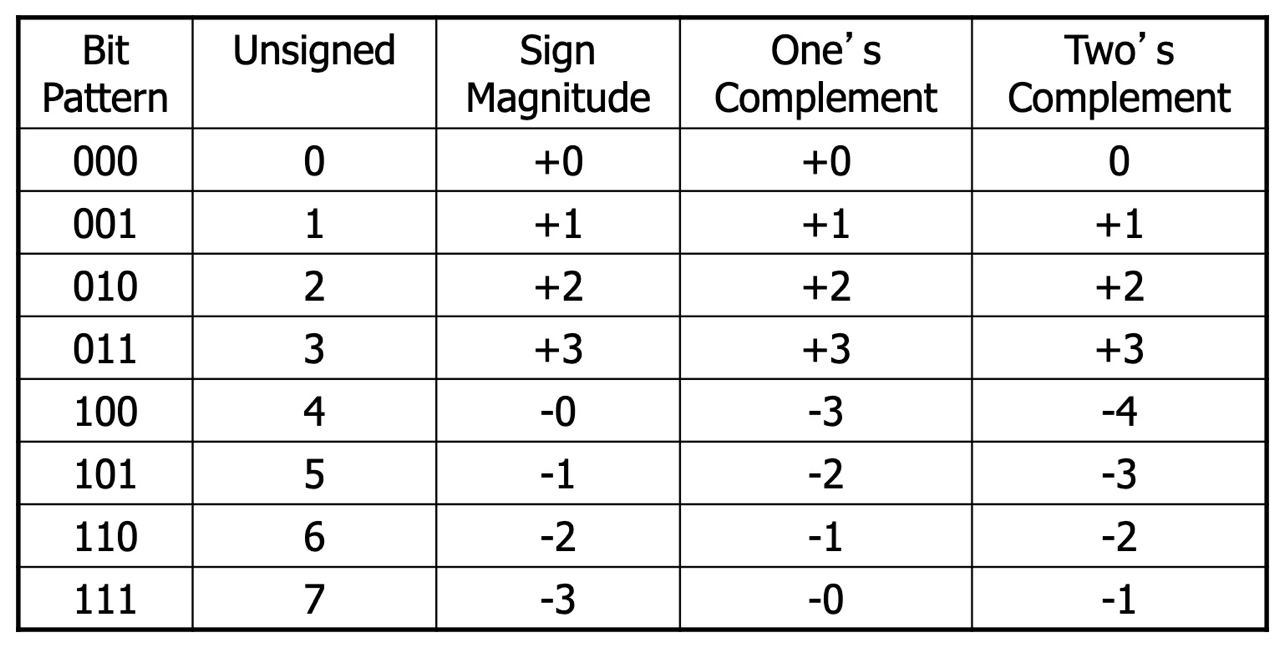
\includegraphics[width=0.9\linewidth]{integer_representation.jpg}
  \begin{itemize}
    \item Sign magnitude and one's complement: Have duplicate zeros
    \item Two's complement: most significant bit is sign bit, 1 if negative 0 if positive
    \item The sign bit is multiplied by -1 and the rest are positive to get value
    \item Negating a two's complement: invert all bits then add 1 to result
    \item Sign extension works because 2 complement's really have infinite 0/1s on the left if positive/negative
    \item Overflow: With w bits, overflow is just (u + v) mod$ 2^w$
    \begin{enumerate}
      \item Hardware does not detect overflow (MIPS: addu, addiu, subu). Onus is on software to check.
      \item Hardware maintains a flag to detect overflow but does nothing.
      \item Hardware raises exception, PC jumps to predefined addr for exception and prior addr is saved for possible recovery. (MIPS: add, addi, sub)
    \end{enumerate}
  \end{itemize}

  \subsection{Pseudo Instructions}
  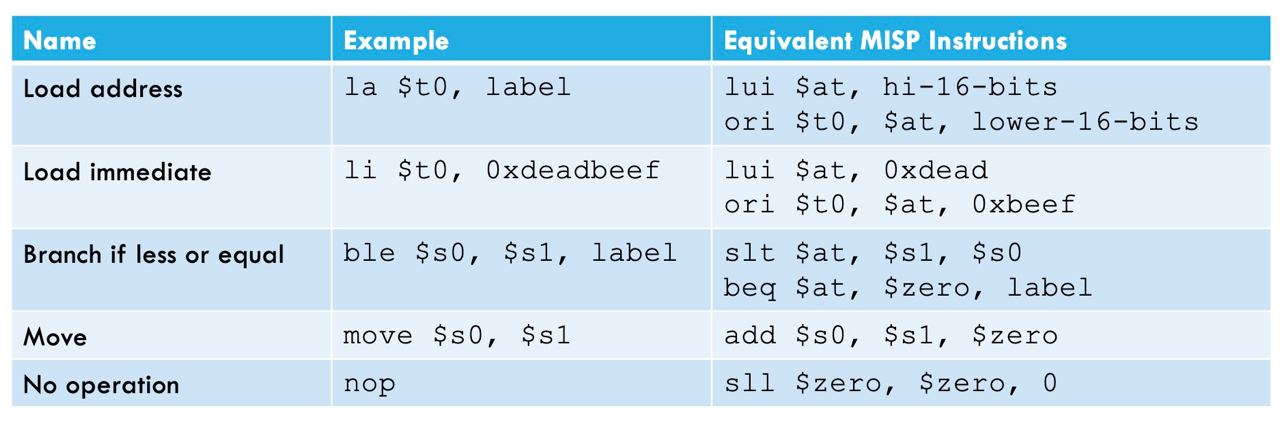
\includegraphics[width=0.9\linewidth]{pseudo_instructions.jpg}\\
  at (register no 1) is the assembler temporary and is reserved by the assembler.

  \subsection{Control instructions}
  \begin{itemize}
    \item In assembly, the branch is typically short distance, range is lower than jump's range.
    \item The reason for padding right with 2 zeros is to make the address divisible by 4. The immediate specifies the i-th multiple of 4, not the i-th address.
    \item Jump addr can be anywhere.
  \end{itemize}

  \subsection{Addressing Modes}
  \begin{itemize}
    \item Memory can be viewed as a single 1-dimensional array of words (32 bits/4 bytes).
    \item MIPS words are aligned: this means we need to times 4 when indexing (see later).
    \item \begin{center}
            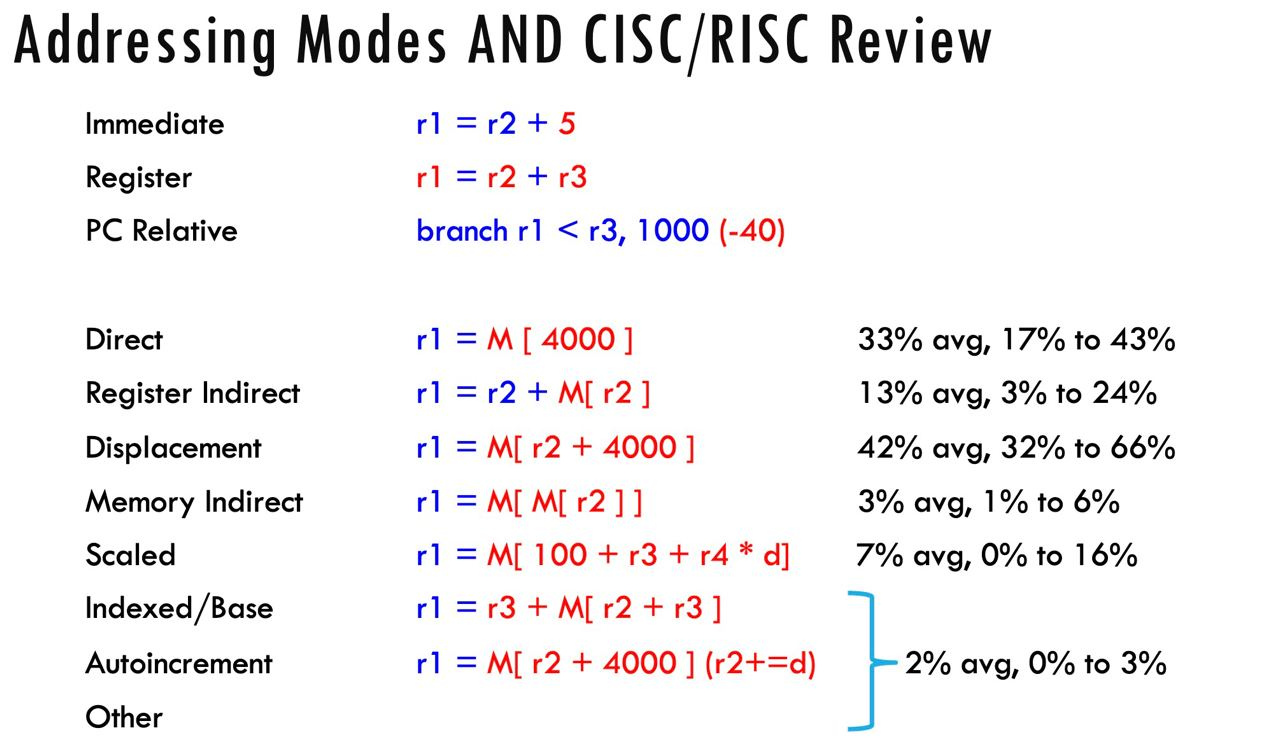
\includegraphics[width=0.75\linewidth]{addressing_modes.jpg}
          \end{center}
    \item Indexed/base, scaled, and memory indirect not supported in MIPS
  \end{itemize}
  
  \subsection{Endianness}
  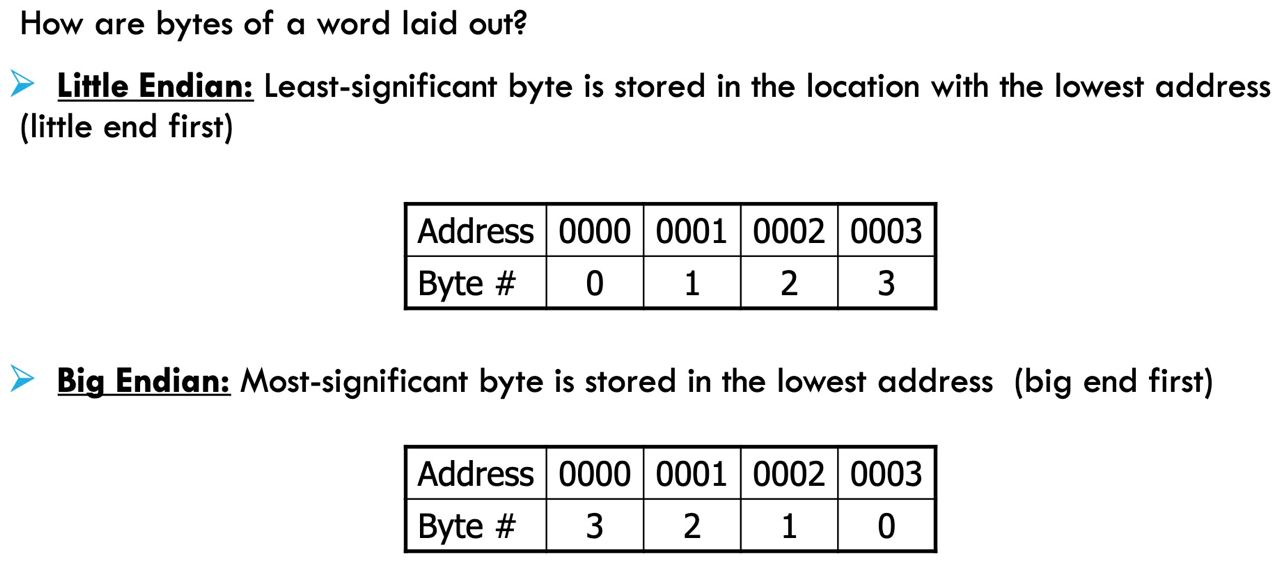
\includegraphics[width=0.9\linewidth]{endianness.jpg}

  \subsection{Registers vs Memory}
  \begin{itemize}
    \item Registers are faster to access than memory as operating on memory requires load and store ops but have comparatively little space.
    \item Space available
    \begin{itemize}
      \item Registers: 32 32 bits registers = 32 * 4 bytes = $2^7$ bytes
      \item Memory: $2^{32}$ bytes ($2^{25}$ times more space)
    \end{itemize}
    \item Compilers use registers as much as possible, spill to memory when required (known as register pressure).
  \end{itemize}

  \subsection{Boolean Algebra}
    \begin{itemize}
      \item NOT 
\includegraphics[width=.25\linewidth]{boolean_not}
      \item AND 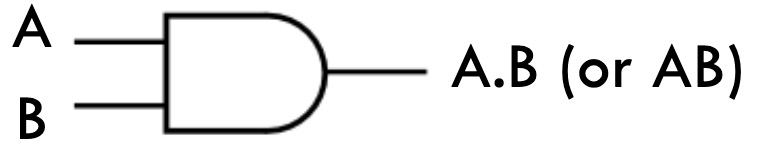
\includegraphics[width=.25\linewidth]{boolean_and}
      \item OR 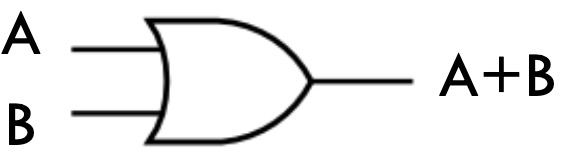
\includegraphics[width=.20\linewidth]{boolean_or}
      \item Boolean Algebra Laws
      \begin{enumerate}
        \item Identity    : A.1 = A, A + 0 = A
        \item Zero and one: A.0 = 0, A + 1 = 1
        \item Inversion   : A.$\overline{A}$ = 0, A + $\overline{A}$ = 1
        \item Idempotence : A.A = A, A + A = A (Useful for generating extra terms)
        \item Commutativity: A.B = B.A, A + B = B + A
        \item Associativity: A.(B.C) = (A.B).C, A + (B + C) = (A + B) + C
        \item Distribution: A + (B.C) = A.B + A.C, A + (B.C) = (A + B).(A + C)
        \item DeMorgan's  : $\overline{A.B}$ = $\overline{A}$ + $\overline{B}$, $\overline{A + B}$ = $\overline{A}$ . $\overline{B}$  
      \end{enumerate}
    \end{itemize}

  \subsection{Performance}
  \begin{itemize}
    \item Million Instructions Per second (MIPS) = $\frac{\text{Instruction count}}{\text{Execution Time} \times 10^6}$
    \item The Iron Law of Computer Performance: $\text{Time} = \text{Instructions} \times \frac{\text{Cycles}}{\text{Instructions}} \times \frac{\text{Time}}{\text{Cycles}}$
    \item $\frac{\text{Cycles}}{\text{Instructions}}$ = CPI (1 / IPC)
    \item $\frac{\text{Time}}{\text{Cycles}}$ = 1/(Clock Frequency)
    \item 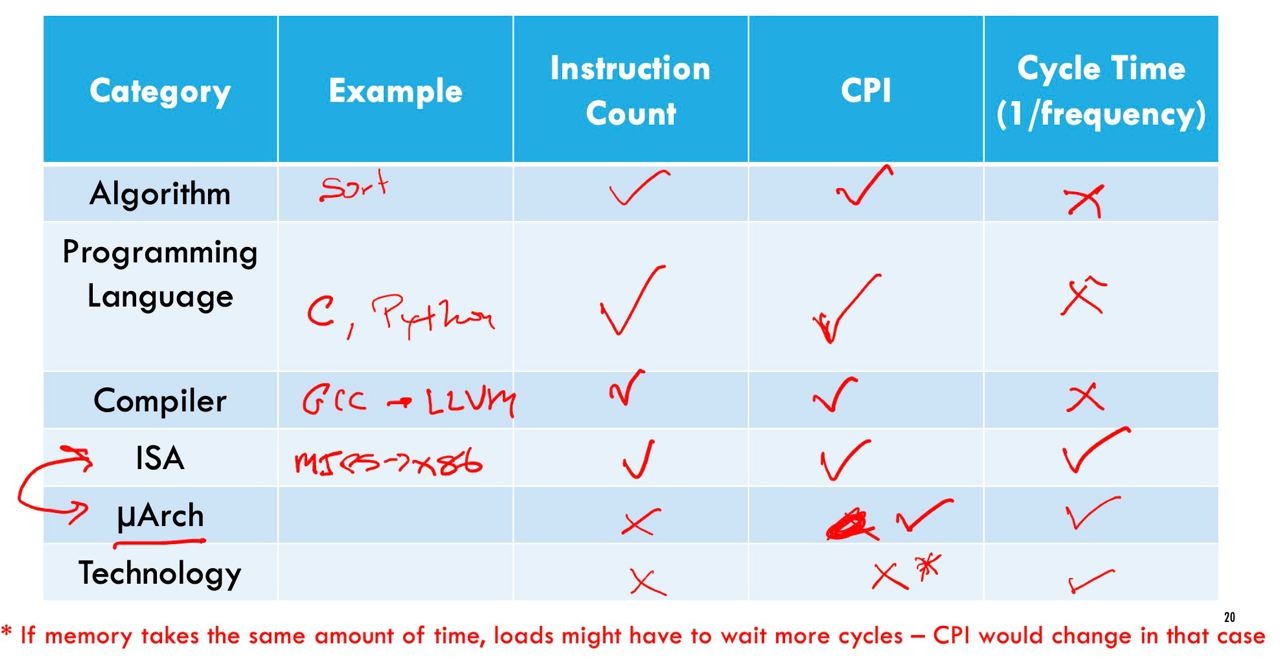
\includegraphics[width=0.75\linewidth]{performance_influence}
    \item 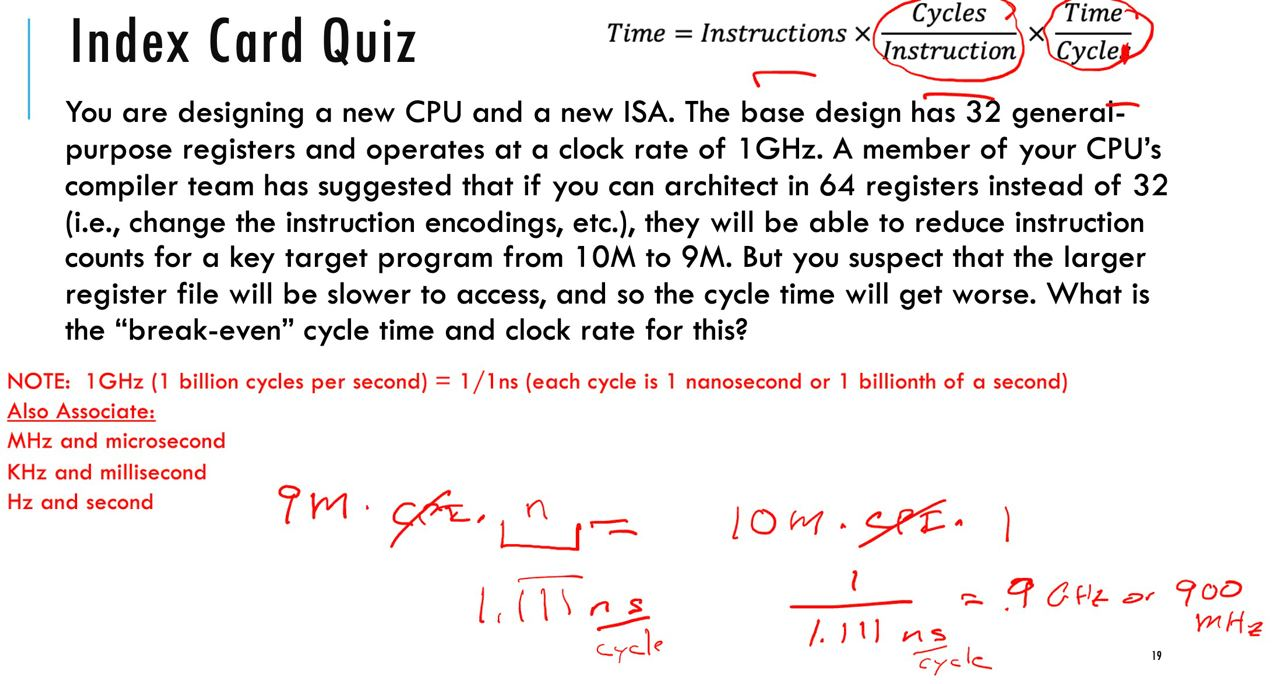
\includegraphics[width=0.75\linewidth]{performance_index_card_quiz}
    \item A cycle is a step. An instruction may take any number of steps. Frequency is the number of cycles per second.
    \item Single cycle forces all instructions to take 1 step hence CPI = 1, at the expense of long cycle time.
  \end{itemize}

  \subsection{Single Cycle Processor}
  \begin{itemize}
    \item Critical path: The clock cycle is determined by the operation that requires the longest time.
    \item Clocking Methodology: Way to prevent unreliable results in computer hardware due to reading/writing at same time.
    \item Clock-Edge: Only read/write on a rising/falling clock edge. Point is it's standardized.
    \item 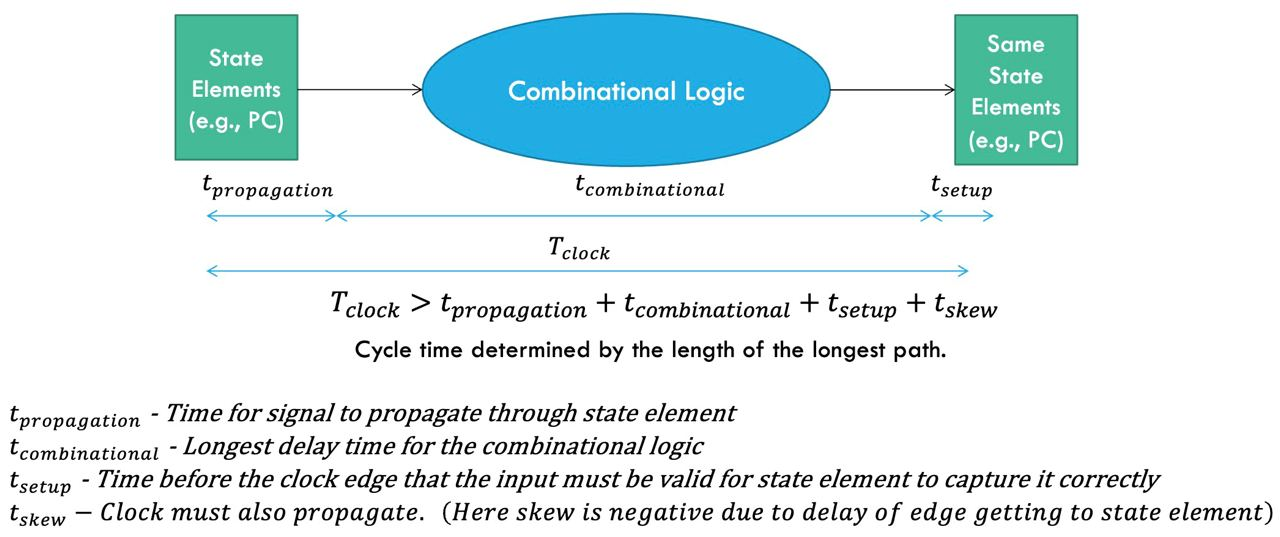
\includegraphics[width=0.75\linewidth]{clock_cycle.jpg}
    \item 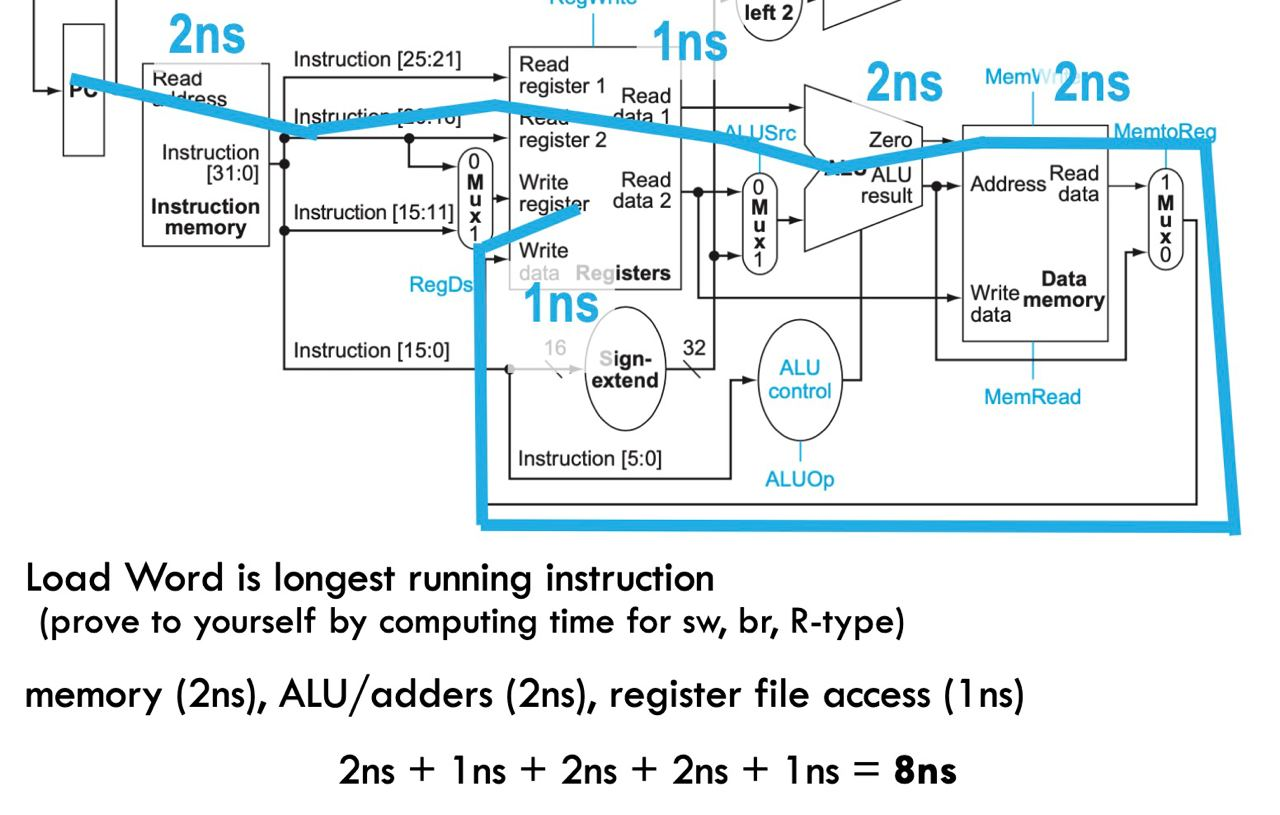
\includegraphics[width=0.75\linewidth]{load_word.jpg}
    \item Combinational circuits: Output solely depends on input. Implements a boolean function.
    \item State elements: Sequential circuits. Output depends on input and state.
    \item 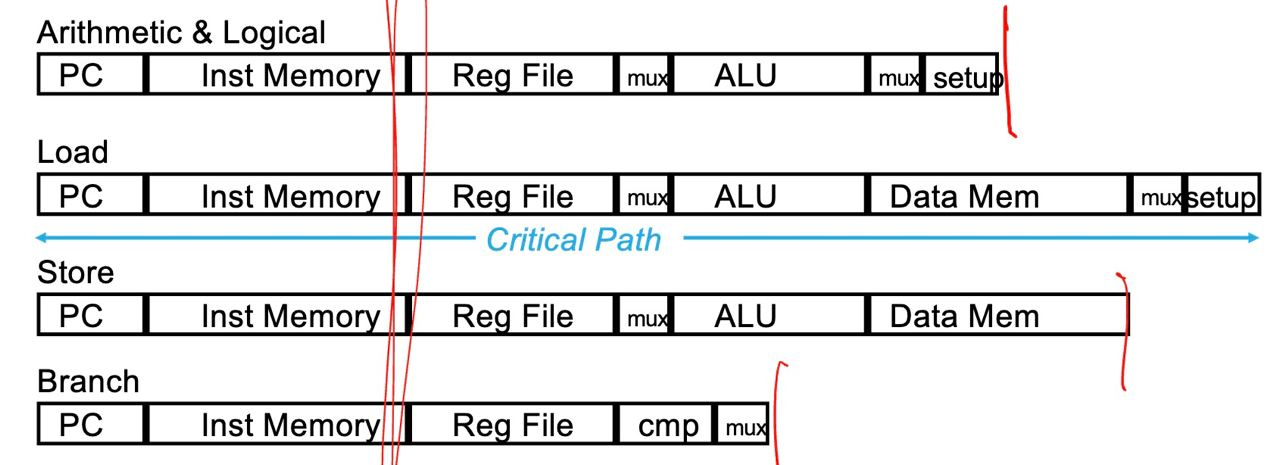
\includegraphics[width=0.75\linewidth]{single_cycle_time_components.jpg}
    \begin{enumerate}
      \item Long cycle time, wasted inefficiency.
      \item Real memory takes a variable amount of time to read and write.
      \item Depending on the ratio of loads/stores/adds/branches, the ideal average time could be much lower.
      \item Haven't even accounted for floating point operations yet which are much slower.
      \item Some units hold value long after job is complete, ALU could be reused, underutilized resources.
    \end{enumerate}
  \end{itemize}
    \subsubsection{Control}
      \begin{itemize}
        \item 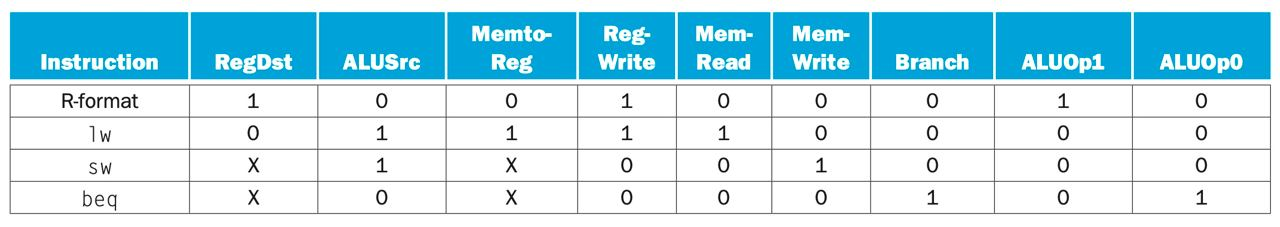
\includegraphics[width=0.95\linewidth]{control_truth_table.jpg}
        \item 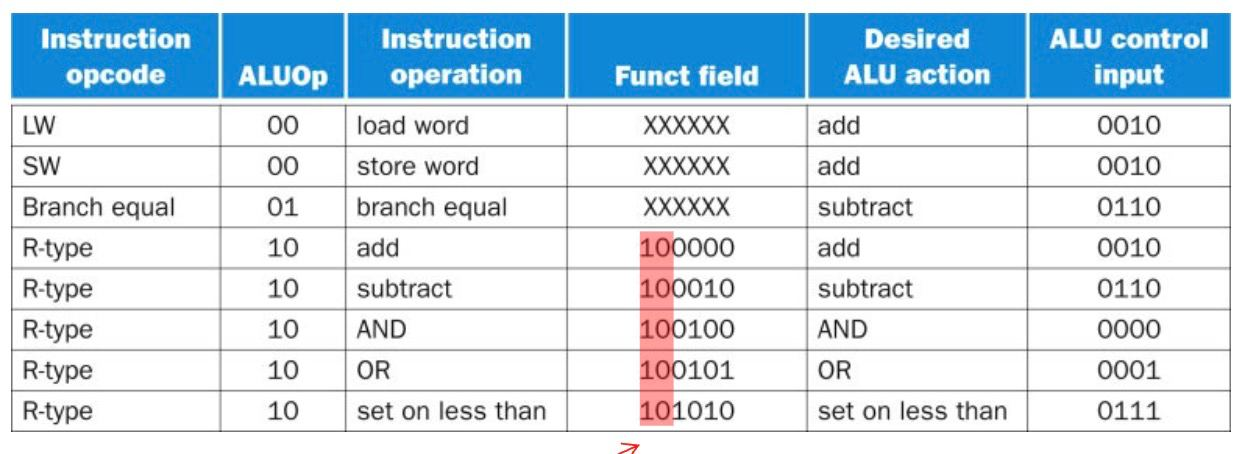
\includegraphics[width=0.95\linewidth]{alu_control_truth_table.jpg}
      \end{itemize}

  \subsection{Multicycle Processor}
      \begin{itemize}
        \item From "The best way to design a machine": Break instructions into steps, one per cycle, such that
        \begin{itemize}
          \item Amount of work in each step is balanced
          \item Restrict each cycle to only one major functional unit
          \item Shorter cycle time
        \end{itemize}
        \item At the end of a cycle, store values for use in later cycles.
        \item Introduce "internal" registers for values between cycles.
        \item Each instruction broken into multiple steps, each step defined as one clock cycle.
        \item 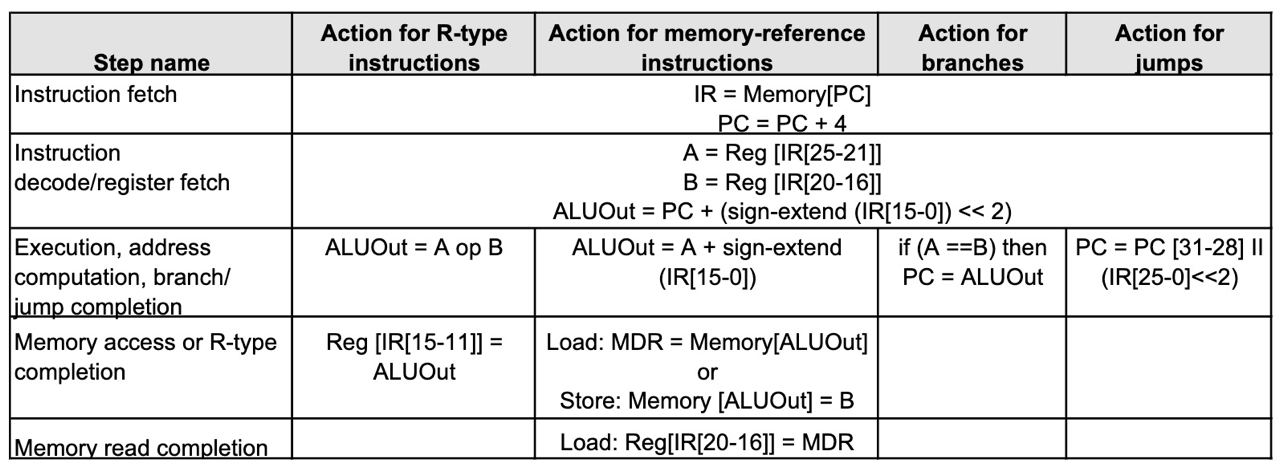
\includegraphics[width=\linewidth]{multicycle_5_stages.jpg}
        \item The control now needs to be specified as a FSM instead of a combinational circuit since there is some state to it.
        \item 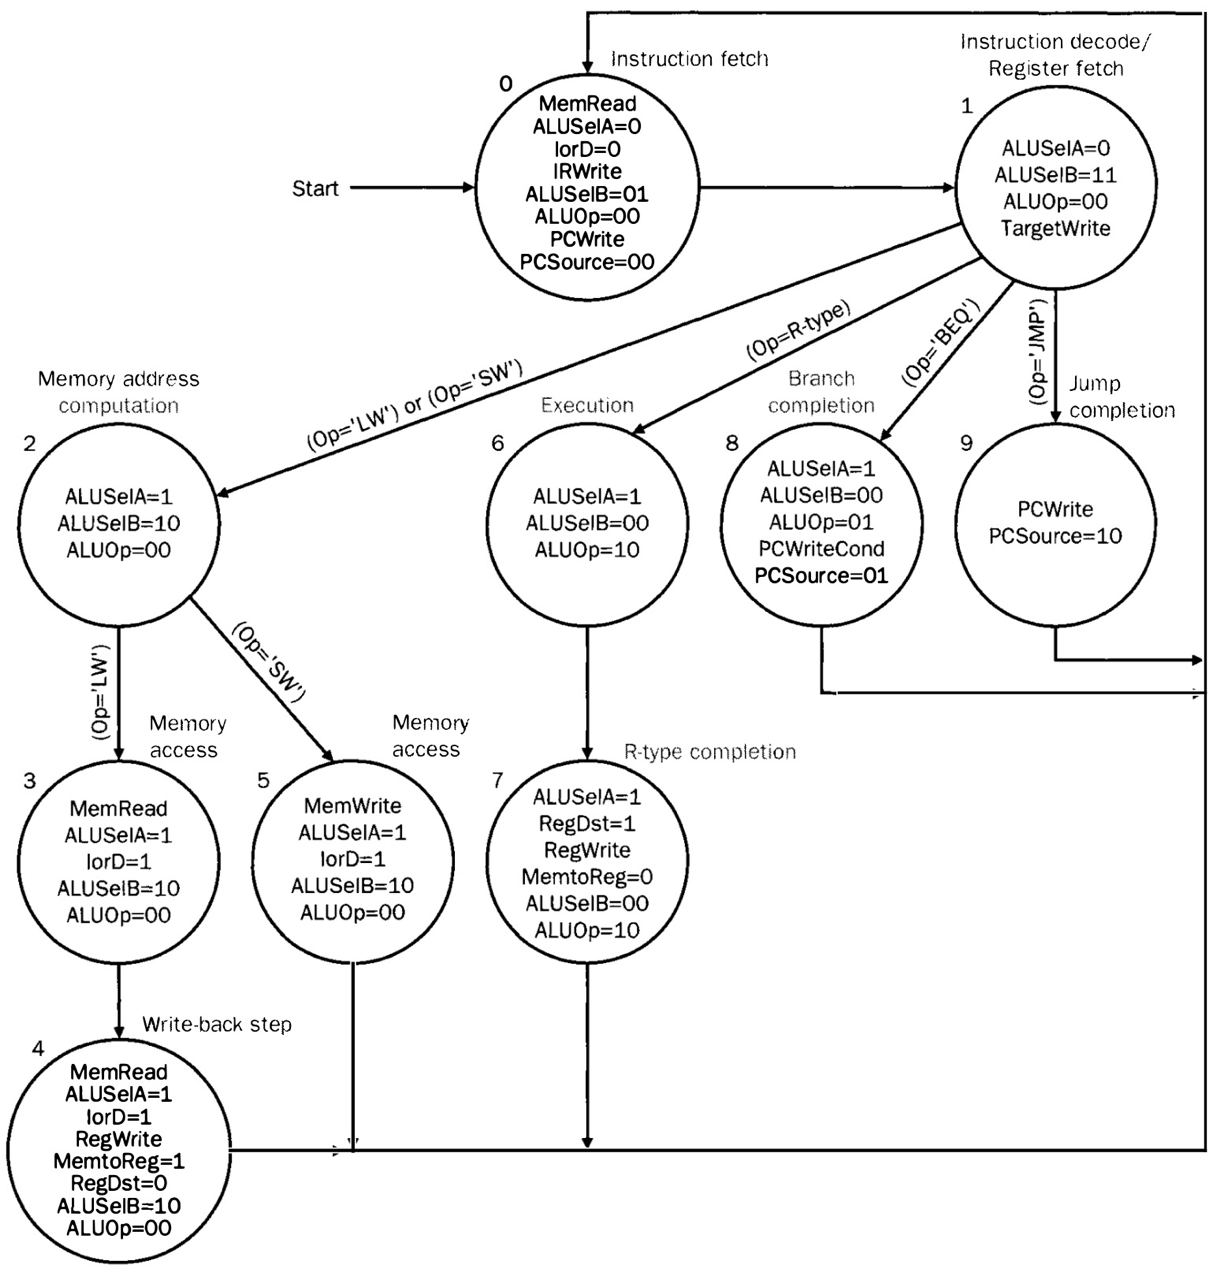
\includegraphics[width=\linewidth]{control_fsm.jpg}
      \end{itemize}

  \subsection{Pipelining}
      \begin{itemize}
        \item Why can't single cycle (from lecture) do pipeline?
        \item Why can't multi cycle (from lecture) do pipeline?
        \item Pipelining increases throughput but does not decrease latency (the time taken to complete one instruction)
        \item We use the same 5 stages as multicycle: IF, ID, EX, MEM, WB.
      \end{itemize}

    \subsubsection{Pipeline Hazards}
      \begin{itemize}
        \item \textbf{Structural Hazard}: Hardware cannot support the combination of instructions that we want to execute in the same clock cycle.
        \item Example: Only a single memory instead of two. Cannot have an instruction access data from memory and another fetch instruction from memory.
        \item \textbf{Data Hazard}: Occurs when the pipeline must be stalled because one step must wait for another to complete. Arises due to RAW dependencies.
        \item Example: add \$s0, \$t0, \$t1; sub \$t2, \$s0, \$t3. 
        \item This can be resolved via \textbf{forwarding/bypassing}. Store the computed value in a buffer and pass to the ALU.
        \item Forwarding is not enough to resolve load data dependency (known as \textbf{load-use data hazard}) since the mem is written one stage after the input. For example, R-type after a lw.
        \item The concept of \textbf{pipeline stall/bubble} where we either detect and reorder or stall.
        \item \textbf{Control Hazard}: The flow of instruction addresses is now what pipeline expects.
        \item Possible approaches include stalling, branch prediction and simply delayed decision (delay slots in MIPS)
      \end{itemize}


  
\end{multicols*}

\end{document}
